\section{Autour de la division}

\definition[]{Vocabulaire}{Une division est constituée d'un \textcolor{violet}{dividende} (celui qui sera divisé), d'un \textcolor{blue}{diviseur} (celui qui divise), d'un \textcolor{red}{quotient} (le résultat) et d'un \textcolor{teal}{reste} (ce qui reste si la division s'arrête à l'unité)\\\vspace{1em}\\
Par exemple avec la division de 19 par 5, on obtient : 
\begin{figure}[H]
    \centering
            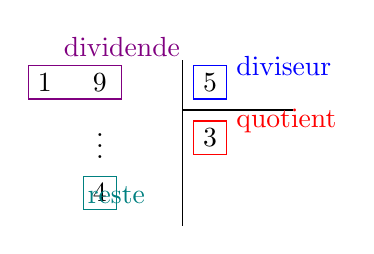
\begin{tikzpicture}[scale=0.7]
                \draw (0,0) node {1} ;
                \draw (1,0) node {9} ;
                \draw [violet] (-0.3,-0.3) rectangle (1.4,0.3) node [above] {dividende} ;
                \draw (2.5,0.4) -- (2.5,-2.6) ;
                \draw (3,0) node {5} ;
                \draw (2.5,-0.5) -- (4.5,-0.5) ;
                \draw (1,-1) node {$\vdots$} ;
                \draw (1,-2) node {4} ;
                \draw (3,-1) node {3};
                \draw [red] (2.7,-1.3) rectangle (3.3,-0.7) node [right] {quotient} ;
                \draw [blue] (2.7,-0.3) rectangle (3.3,
                0.3) node [right] {diviseur} ;
                \draw [teal] (0.7,-2.3) rectangle (1.3,
                -1.7) node [below = .3] {reste} ;
            \end{tikzpicture}
    \end{figure}
Qui peut aussi s'écrire \textcolor{violet}{19} = \textcolor{blue}{5} $\times$ \textcolor{red}{3} + \textcolor{teal}{4}.
}

\propriete[
    \exmplist
        {27 $:$ 4 devient :\\ \opdiv[shiftintermediarysymbol=\textcolor{gray}{0},displayintermediary=all]{27}{4}}
        {33 $:$ 4 devient :\\ \opdiv[shiftintermediarysymbol=\textcolor{gray}{0},displayintermediary=all]{33}{4}}
        {114 $:$ 6 devient :\\ \opdiv[shiftintermediarysymbol=\textcolor{gray}{0},displayintermediary=all]{114}{6}} 
]
{Poser une division}
{On va ici poser la multiplication 131 $\times$ 3.\\\vspace{1em}\\
\begin{minipage}{0.7\textwidth}    
On pose les deux nombres à diviser, le \textcolor{blue}{diviseur} à droite et le \textcolor{violet}{dividende} à gauche.  
\end{minipage}
\hfill
\begin{minipage}{0.22\textwidth}
    \begin{figure}[H]
    \centering
        \resizebox{\textwidth}{!}{
            \begin{tikzpicture}[scale=0.7]
                \draw [violet] (0,0) node {1} ;
                \draw [violet] (1,0) node {3} ;
                \draw [violet] (2,0) node {1} ;
                \draw (2.5,0.4) -- (2.5,-2.6) ;
                \draw [blue] (3,0) node {3} ;
                \draw (2.5,-0.5) -- (4.5,-0.5) ;
            \end{tikzpicture}
        }
    \end{figure}
\end{minipage}
\\\vspace{1em}\\
\begin{minipage}{0.7\textwidth}    
    On regarde si le premier chiffre du dividende est plus grand que le diviseur. Ici, 1 est plus petit que 3. On regarde donc le nombre formé par les deux premiers chiffres du dividende. C'est bon, 13 est plus grand que 3, on peut commencer à diviser. Dans 13, \textcolor{teal}{il y a 4 fois 3} car \textcolor{red}{$4\times 3=12$}. \textcolor{blue}{On peut mainteant faire la soustraction 13-12=1}
\end{minipage}
\hfill
\begin{minipage}{0.22\textwidth}
    \begin{figure}[H]
    \centering
        \resizebox{\textwidth}{!}{
            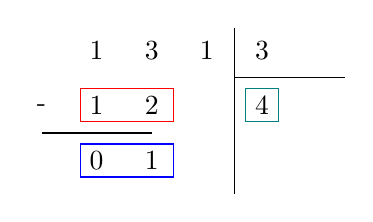
\begin{tikzpicture}[scale=0.7]
                \draw (0,0) node {1} ;
                \draw (1,0) node {3} ;
                \draw (2,0) node {1} ;
                \draw (2.5,0.4) -- (2.5,-2.6) ;
                \draw (3,0) node {3} ;
                \draw (2.5,-0.5) -- (4.5,-0.5) ;
                \draw (3,-1) node {4} ;
                \draw [teal] (2.7,-1.3) rectangle (3.3,-0.7)  ;
                \draw [red] (-0.3,-1.3) rectangle (1.4,-0.7) ;
                \draw (-1,-1) node {-} ;
                \draw (0,-1) node {1} ;
                \draw (1,-1) node {2} ;
                \draw (-1,-1.5) -- (1,-1.5) ;
                \draw (0,-2) node {0} ;
                \draw (1,-2) node {1} ;
                \draw [blue] (-0.3,-2.3) rectangle (1.4,-1.7) ;
            \end{tikzpicture}
        }
    \end{figure}
\end{minipage} \\ \vspace{1em}\\
\begin{minipage}{0.7\textwidth}    
    \textcolor{red}{On descend ensuite le chiffre suivant}, et on recommence la division. Dans 11, il y a \textcolor{teal}{3 fois 3 car $3\times 3=9$}. Et \textcolor{blue}{11-9=2}
\end{minipage}
\hfill
\begin{minipage}{0.22\textwidth}
    \begin{figure}[H]
    \centering
        \resizebox{\textwidth}{!}{
            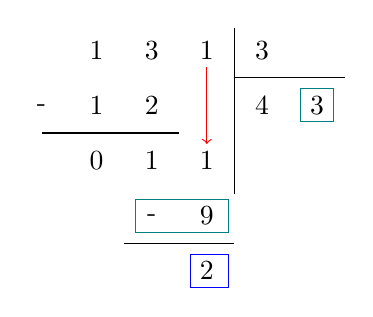
\begin{tikzpicture}[scale=0.7]
                \draw (0,0) node {1} ;
                \draw (1,0) node {3} ;
                \draw (2,0) node {1} ;
                \draw (2.5,0.4) -- (2.5,-2.6) ;
                \draw (3,0) node {3} ;
                \draw (2.5,-0.5) -- (4.5,-0.5) ;
                \draw (3,-1) node {4} ;
                \draw (4,-1) node {3} ;
                \draw [teal] (3.7,-1.3) rectangle (4.3,-0.7)  ;
                \draw (-1,-1) node {-} ;
                \draw (0,-1) node {1} ;
                \draw (1,-1) node {2} ;
                \draw (-1,-1.5) -- (1.5,-1.5) ;
                \draw (0.5,-3.5) -- (2.5,-3.5) ;
                \draw (0,-2) node {0} ;
                \draw (1,-2) node {1} ;
                \draw (2,-2) node {1} ;
                \draw (2,-3) node {9} ;
                \draw (2,-4) node {2} ;
                \draw (1,-3) node {-} ;
                \draw [red,->] (2,-0.3) -- (2,-1.7) ;
                \draw [teal] (0.7,-3.3) rectangle (2.4,-2.7) ;
                \draw [blue] (1.7,-4.3) rectangle (2.4,-3.7) ;
            \end{tikzpicture}
        }
    \end{figure}
\end{minipage}
Comme 2 est plus petit que 3 et qu'il n'y a pas de chiffre de plus à descendre, la division est terminée. La division de 131 par 3 donne donc 43, et il reste 2.
}

\propriete[]{Division non entiere}{Si on veut ne veut pas de reste, on peut obtenir un résultat à virgule.\\Reprenons le calcul précédent : \\
\begin{minipage}{0.7\textwidth}    
    Dans ce cas, \textcolor{red}{on rajoute ,0 à la suite du dividende} et \textcolor{blue}{une virgule à la suite du quotient.}
\end{minipage}
\hfill
\begin{minipage}{0.22\textwidth}
    \begin{figure}[H]
    \centering
        \resizebox{\textwidth}{!}{
            \begin{tikzpicture}[scale=0.7]
                \draw (0,0) node {1} ;
                \draw (1,0) node {3} ;
                \draw (2,0) node {1} ;
                \draw [red] (2.5,-0.2) node {,} ;
                \draw [red] (3,0) node {0} ;
                \draw (4.5,0.4) -- (4.5,-2.6) ;
                \draw (5,0) node {3} ;
                \draw (4.5,-0.5) -- (7.5,-0.5) ;
                \draw (5,-1) node {4} ;
                \draw (6,-1) node {3} ;
                \draw [blue] (6.5,-1.2) node {,} ;
                \draw (-1,-1) node {-} ;
                \draw (0,-1) node {1} ;
                \draw (1,-1) node {2} ;
                \draw (-1,-1.5) -- (1.5,-1.5) ;
                \draw (0.5,-3.5) -- (2.5,-3.5) ;
                \draw (0,-2) node {0} ;
                \draw (1,-2) node {1} ;
                \draw (2,-2) node {1} ;
                \draw (2,-3) node {9} ;
                \draw (2,-4) node {2} ;
                \draw (1,-3) node {-} ;
            \end{tikzpicture}
        }
    \end{figure}
\end{minipage}
\begin{minipage}{0.7\textwidth}    
    Ensuite, on redescend le 0, et on continue la division.\\
    \textcolor{blue}{Dans 20, il y a 6 fois 3}, et \textcolor{teal}{20-18=2}
\end{minipage}
\hfill
\begin{minipage}{0.22\textwidth}
    \begin{figure}[H]
    \centering
        \resizebox{\textwidth}{!}{
            \begin{tikzpicture}[scale=0.7]
                \draw (0,0) node {1} ;
                \draw (1,0) node {3} ;
                \draw (2,0) node {1} ;
                \draw (2.5,-0.2) node {,} ;
                \draw (3,0) node {0} ;
                \draw (4.5,0.4) -- (4.5,-6.6) ;
                \draw (5,0) node {3} ;
                \draw (4.5,-0.5) -- (7.5,-0.5) ;
                \draw (5,-1) node {4} ;
                \draw (6,-1) node {3} ;
                \draw [blue] (7,-1) node {6} ;
                \draw (6.5,-1.2) node {,} ;
                \draw (-1,-1) node {-} ;
                \draw (0,-1) node {1} ;
                \draw (1,-1) node {2} ;
                \draw (-1,-1.5) -- (1.5,-1.5) ;
                \draw (0.5,-3.5) -- (2.5,-3.5) ;
                \draw (0,-2) node {0} ;
                \draw (1,-2) node {1} ;
                \draw (2,-2) node {1} ;
                \draw (2,-3) node {9} ;
                \draw (2,-4) node {2} ;
                \draw (1,-3) node {-} ;
                \draw (3,-4) node {0} ;
                \draw [blue] (3,-5) node {8} ;
                \draw [blue] (2,-5) node {1} ;
                \draw [blue] (1,-5) node {-} ;
                \draw (0.5,-5.5) -- (3.5,-5.5) ;
                \draw [teal] (3,-6) node {2} ;
            \end{tikzpicture}
        }
    \end{figure}
\end{minipage}
\\ \vspace{1em}\\
Et on peut continuer autant d'étapes que nécessaire, sans oublier de rajouter et descendre un 0 à chaque fois.
}

\begin{comment}
\propriete[\rmq Si on a un nombre à virgule, on peut donc multiplier à la fois le diviseur et le dividende par 10 (et décaler leurs virgules vers la droite) jusqu'à ne plus avoir de virgule. \\\vspace{1em}\\
\exmpl 33,4 : 2 devient alors : \\ \opdiv{33.4}{2}]{Division et multiplication par 10}{Le résultat d'une division reste le même si on multiplie (ou divise) le diviseur et le dividende par 10.}
\end{comment}

\section{Divisibilité}

\definition[\exmpl\begin{itemize}
    \item 15 est divisible par 5
    \item 30 est divisible par 3
    \item 15 n'est pas divisible par 4
\end{itemize}]{divisible}{On dit qu'un nombre est divisible par un autre si le reste de sa division par ce nombre est égal à 0}

\propriete[]{Critères de divisibilité}{Un nombre est divisible par : 
\begin{itemize}
    \item 2 s'il se termine par 0 ; 2 ; 4 ; 6 ou 8.
    \begin{itemize}
        \item \textcolor{gray}{122228 est divisible par 2 car il se termine par 8}
    \end{itemize}
    \item 3 si la somme de ses chiffre est divisible par 3.
    \begin{itemize}
        \item \textcolor{gray}{132465 est divisible par 3 car 1+3+2+4+6+5=21 qui est divisible par 3}
    \end{itemize}
    \item 4 si le nombre formé par ses deux derniers chiffres est divisible par 4.
    \begin{itemize}
        \item \textcolor{gray}{122228 est divisible par 4 car 28 est divisible par 4}
    \end{itemize}
    \item 5 s'il se termine par 0 ; ou 5.
    \begin{itemize}
        \item \textcolor{gray}{12225 est divisible par 5 car il se termine par 5}
    \end{itemize}
    \item 6 s'il est divisible par 2 et par 3.
    \begin{itemize}
        \item \textcolor{gray}{12222 est divisible par 2 car il se termine par 2}
        \item \textcolor{gray}{12222 est divisible par 3 car 1+2+2+2+2=9}
        \item \textcolor{gray}{Donc, 12222 est divisible par 6}
    \end{itemize}
    \item 9 si la somme de ses chiffre est divisible par 9.
    \begin{itemize}
        \item \textcolor{gray}{981 est divisible par 9 car 9+8+1=18 qui est divisible par 9}
    \end{itemize}
\end{itemize}}

